\chapter{Track Reconstruction}
\label{sec:track}
	The~first stage of our reconstruction algorithm is the~reconstruction of the~track of the~primary particle (either an~electron or a~positron). The~results of this step are then used to determine the~energy of the~particle (see Section~\ref{sec:energy}).
	
	\textbf{First Attempts} at a~track reconstruction were made using the~standard approach. Here, we assume that the~readout coordinates ($x'$,~$y'$,~$t$) are known exactly, neglecting the~pads and time bins. In a~standard \ac{TPC} (with parallel fields), we only need to reconstruct the~$z$~coordinate from drift time using the~known drift velocity.
	
	Reconstruction using the~\textbf{Ionization Electron Map} (from now on referred to as \emph{the~map}) uses a~simulation of the~drift of secondary (ionization) electrons within the~detector volume. This simulation can then be used to interpolate the~initial position of the~secondary electrons. First attempts neglect the~pads.
	
	We used the~map for reconstruction in two different ways. The~first one uses gradient descent search along with trilinear interpolation (see Section~\ref{sec:trilin}) in the~map. The~second method uses interpolation in the~irregular inverse grid with a~linear polynomial.
	
	The~\textbf{Discrete Reconstruction} uses the~map; instead of reconstructing the~exact position of each electron, we reconstruct the~center of each hit pad with the~time corresponding to the~midpoint of the~time bin. The~number of electrons in each \ac{TPC}~bin (consisting of the~pad and the~time bin) is counted and used as a~charge in the~energy reconstruction.
	
	\section{First Attempts}
	\label{sec:trackfirst}
		As the~first step, we decided to try to reconstruct an~electron track with a~special set of initial parameters. The~origin of the~particle is given by the~origin of our coordinate system. The~initial direction is given by the~positive $x$~axis. This means the~magnetic field of our detector is perpendicular to the~momentum of our particle at all times, and we can reduce the~problem to two-dimensional space. We use a~track simulated using the~microscopic simulation (see Section~\ref{sec:microsim}) with a~kinetic energy of 8~MeV. The~gas composition used in this simulation is 90\%~Ar~+~10\%~CO$_2$.
		
		In this first approach to the~reconstruction of the~track, we decided to use the~common method used in a~standard \ac{TPC}. This will allow us to explore the~significance of the~atypical behavior in our \ac{OFTPC}. Additionally, we assume the~readout is continuous to further simplify the~problem. In this approximation, we reconstruct the~initial position of each ionization electron.
		
		The~reconstruction is then defined by the~following relations between the~coordinates of the~detector space and the~readout space (see Section~\ref{sec:coor}):
			\begin{eqnarray}
				x = x',\\
				y = y',\\
				z = v_d t,
			\end{eqnarray}
		where $v_d$ is the~drift velocity of electrons in the~given gas mixture. At a~phenomenological level, this velocity can be considered a~function of the~electric field~$\bm{E}$ and the~magnetic field~$\bm{B}$:
			\begin{equation}
				v_d = v_d(\bm{E},\bm{B}).
			\end{equation}
		\textcolor{red}{Taken from Garfield user manual.} The~Garfield++ toolkit uses this fact to accelerate their drift simulation with non-microscopic approaches. Since we assume a~uniform electric field in our detector and we want to neglect the~effect of our unusual magnetic field, we consider the~drift velocity to be constant in this scenario. We then approximate this velocity by fitting the~dependence $z(t)$ taken from the~simulated ionization electrons. \textcolor{red}{This is in one of the~provisional figures. Also, this description is not completely accurate; in reality, we fit t1:8-y0 with a1*x+a0 and then invert this and use 8-y0 = b1*t1+b0 (old coordinates); b1=1/a1 functions as the~drift velocity. Maybe also define this 8-z variable as an~alternative to z in Section~\ref{sec:coor} and then use it when correcting this.}
		
		\textcolor{red}{Later, in a~commit after this, I plotted some residues (provisional figure), which could be useful, but for some reason they are residuals from a~spline fit of the~track?! Probably redo this without the~spline fit; just explore the~difference in individual points.}
		
		\begin{figure}[H]
			\centering
			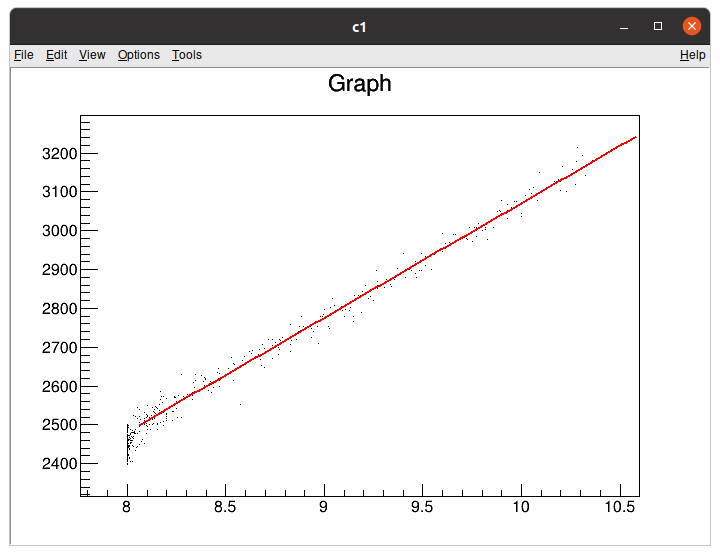
\includegraphics[width=0.5\textwidth]{9010_zt.png}
			\caption{Dependence of the~drift time on the~$z$~coordinate in 90~\%~argon and 10~\%~CO$_2$ atmosphere, fitted with a~linear function. The~fitted function gives us the~average drift velocity in the~gas and can be used for rough reconstruction in our \ac{TPC}. \textcolor{red}{Swap for better image with axis labels, etc. Maybe write the~fitted equation.}}
			\label{fig:9010zt}
		\end{figure}
		
		\begin{figure}[H]
			\centering
			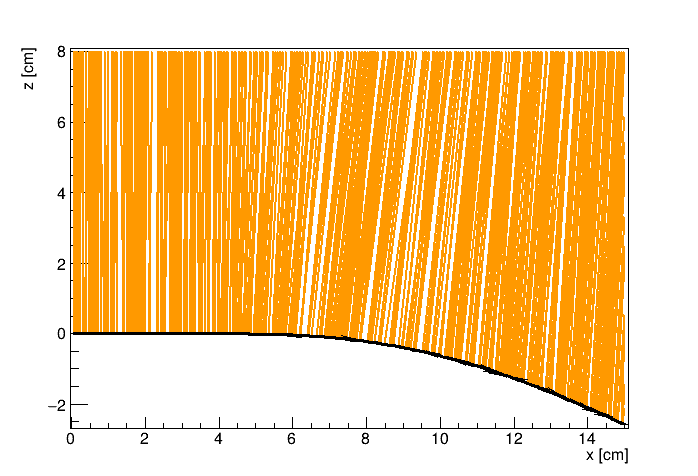
\includegraphics[width=0.5\textwidth]{9010_xz.png}
			\caption{First attempt at a~track reconstruction using only the~drift velocity. This approach works well in a~standard \ac{TPC} (\textcolor{red}{ideally cite some source?}). 90~\%~argon and 10~\%~CO$_2$ atmosphere. \textcolor{red}{Swap for better image, correct coordinates.}}
			\label{fig:9010xz}
		\end{figure}
		
		\begin{figure}[H]
			\centering
			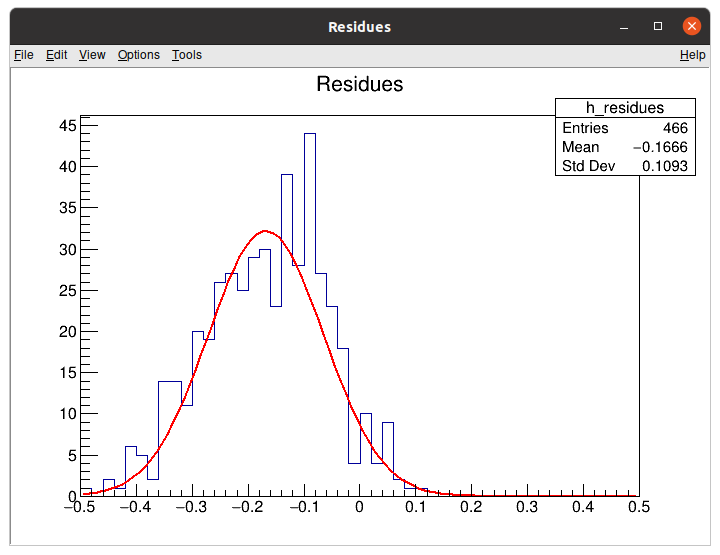
\includegraphics[width=0.5\textwidth]{9010_res.png}
			\caption{First attempt at a~track reconstruction using only the~drift velocity, residues. \textcolor{red}{Swap for better image, correct coordinates. What's causing the~shift? Explain details.}}
			\label{fig:9010res}
		\end{figure}
	
	\section{Ionization Electron Map}
	\label{sec:map}
		Inside an~\ac{OFTPC}, the~drift of the~secondary (ionization) electrons is significantly affected by its magnetic field. We need to take this into account for accurate reconstruction. In the~first approximation, we assume a~continuous readout (i.e., we neglect pads). We can then reconstruct the~original position of each ionization electron using its readout coordinates. For this purpose, we use the~ionization electron map.
		
		The~ionization electron map is a~mapping from the~detector space to the~readout space. It tells us what readout coordinates $(x',y',t)$ we can expect on average for an~ionization electron created in the~detector coordinates $(x,y,z)$. \textcolor{red}{More precisely it is a~mapping to the~distributions on the~readout space; we can simplify this as only the means $\overbar{\mathcal{M}}$ and the covariance matrices $\mathcal{M}_\text{cov}$, assuming Gaussian distribution.}
			\begin{equation}
				\mathcal{M}: \mathcal{D} \longrightarrow \mathcal{R},\; (x,y,z) \longmapsto (x',y',t).
			\end{equation}
		To get an~approximation of this mapping, we simulate the~drift of ionization electrons generated on a~regular grid inside the~volume of our \ac{OFTPC} (\textcolor{red}{actually, we do not take the~detector walls into account and simulate even outside of the~\ac{OFTPC}}). It is also useful to simulate multiple (100 in our case) electrons originating from the~same position so we can get a~better approximation of the~average drift and its variance. In order to get accurate results, we use the~microscopic simulation of these electrons described in Section~\ref{sec:microsim}. When evaluating the~map inside the~grid, we use trilinear interpolation (see Section~\ref{sec:trilin}). From now on, we will denote this interpolated simulation with the~same symbol $\mathcal{M}$.
		
		Finally, we need to invert the~map to get the~original detector coordinates $(x,y,z)$ for the~given readout coordinates $(x',y',t)$. In our case, we can reasonably assume that the mapping $\overbar{\mathcal{M}}$ is one-to-one (as seen in the simulations). We implemented two methods for this purpose: the gradient descent search (Section~\ref{sec:grad}) and interpolation in the~inverse grid (Section~\ref{sec:interpol}).
		
		\textcolor{red}{If we wanted to further improve this, taking into account the whole map $\mathcal{M}$, we could make an 'inverse map' from $\mathcal{R}$ to distributions on $\mathcal{D}$. We could probably achieve this by taking the~normalized probability density of an~electron with initial coordinates $(x,y,z)$ having readout coordinates $(x',y',t)$. If we fix $(x',y',t)$, we get an~unnormalized probability density $f(x,y,z) = \mathcal{M}_{(x,y,z)}(x',y',t)$ (assuming that all initial coordinates are a~priori equally likely). This could potentially improve the~discrete reconstruction if we take the~mean value of this probability density across the pad and time bin}
			\begin{equation}
				\color{red}
				f_\text{pad, bin}(x,y,z) = \frac{1}{A_\text{pad} \Delta t_\text{bin}} \int_\text{pad, bin} \mathcal{M}_{(x,y,z)}(x',y',t) \text{d}x'\text{d}y'\text{d}t
			\end{equation}
		\textcolor{red}{and using it for a~likelihood fit instead of using least squares. This still assumes that all initial coordinates are equally likely which is clearly not the~case for a~primary particle track. In the future, we could even use the~fast track simulation with the~map (should be possible to make around 1000 tracks per minute per core with current settings), create a~big set of tracks with reasonable parameters and use these to get an~approximation of the probability distribution of the~detector response. Some approximations would be necessary when interpreting the~data to decrease the~degrees of freedom of this distribution (we would have to pick a set of parameters and assume that some of them are independent). This could give us an~idea about the~best achievable resolution (how significantly will the~detector response differ for a~given change in energy). If the~difference is significant, we could try to further improve the~likelihood fit.}
		
		The~simulation of the~map is a~computationally heavy task. For this reason, we use a~grid MetaCentrum \textcolor{red}{(citation)} to parallelize it. At first, this was done by evenly distributing the~simulated electrons across the~individual jobs. This was used in the~first simulation with only one electron per vertex in the~regular grid with the~spacing of one centimeter. 
		
		Later, a~better approach was implemented, accounting for the~varying lengths of the~drift of individual electrons. If we index the~electrons in the~order of increasing coordinates $y,x,z$ (\textcolor{red}{picture?}), we can express the~number~$n_l$ of full XY~layers (i.e., electrons with the~same $z$~coordinate) of electrons with index less than or equal to $i$
			\begin{equation}
				n_l(i) = \left\lfloor\frac{i}{n_{xy}}\right\rfloor,
			\end{equation}
		where $n_{xy}$ is the~number of electrons in each XY~layer calculated simply by counting the~electrons that satisfy boundary conditions for $x$~and~$y$. \textcolor{red}{These conditions should be mentioned above; sector condition + maximal $x$ value.} The~number of electrons remaining in the~top layer is then
			\begin{equation}
				n_r(i) = i\!\!\!\!\mod n_{xy}.
			\end{equation}
		Finally, we can calculate the~sum of the~drift gaps of electrons up to index~$i$
			\begin{equation}
				d_\text{sum} = (z_\text{max}-z_\text{min})n_{xy}n_l-\frac{n_l(n_l-1)}{2}n_{xy}l+n_r(z_\text{max}-z_\text{min}-n_l l).
			\end{equation}
		We then use a~binary search algorithm to find the~maximum index $i$ such that the value of this sum is less than the~fraction $\frac{\text{job id}}{\text{max job id}}$ of the~total sum. This way we obtain the~minimal and the~maximal index of electrons simulated in the~given job.
		\textcolor{red}{The~spacing $l$ should be probably defined above + picture of the~simulating grid (1 layer). zmin zmax also}
		
		\textcolor{red}{After the~simulation of the~map, we calculate the~mean readout coordinates assuming Gaussian distribution (i.e., we use averages). We also calculate standard deviations in a~later commit, should be upgraded to the~covariance matrix. We never actually plotted the~distributions we get when simulating the~same electron multiple times, so we do not know if our assumptions are accurate (could also run some statistical test to see how well the~Gaussian distribution fits).}
		
		\textcolor{red}{The~map is then stored in a~\textit{Field}, a~custom class template, could expand on that. Maybe earlier, since the~same template is used for the~magnetic field.}
		
		\textcolor{red}{Could insert a~table here describing all 4 simulations of the~map (gas composition, spacing, etc.). Simulation inside one sector (at first double angle). Extra space on the~sensor. Edge cases not taken into account (TPC wall). Using qsub (not sure if important). Add plots of distortion of the~coordinates. Could also do these~plots in a~different way (e.g., drawing all the~endpoints of each ionization electron or some error ellipse plot).}
		
		\textcolor{red}{Images to add (comparison of both simulations):}
		\begin{itemize}
			\item \textcolor{red}{3D visualization of the map, simulation example}
			\item \textcolor{red}{$z$ vs. $t$ plot}
			\item \textcolor{red}{XY plane distortion for different $z$ values; with arrows and error bars, for all $z$-layers with different colors}
			\item \textcolor{red}{XZ plane ($y = 0$) distortion in $x$ (maybe not necessary?)}
			\item \textcolor{red}{XT plot ($y = 0$) showing (small) distortion in drift times}
		\end{itemize}
		
		\textcolor{red}{More images:}
		\begin{itemize}
			\item \textcolor{red}{Residuals of the~continuous readout reconstruction.}
		\end{itemize}		
		
		\begin{figure}[H]
			\centering
			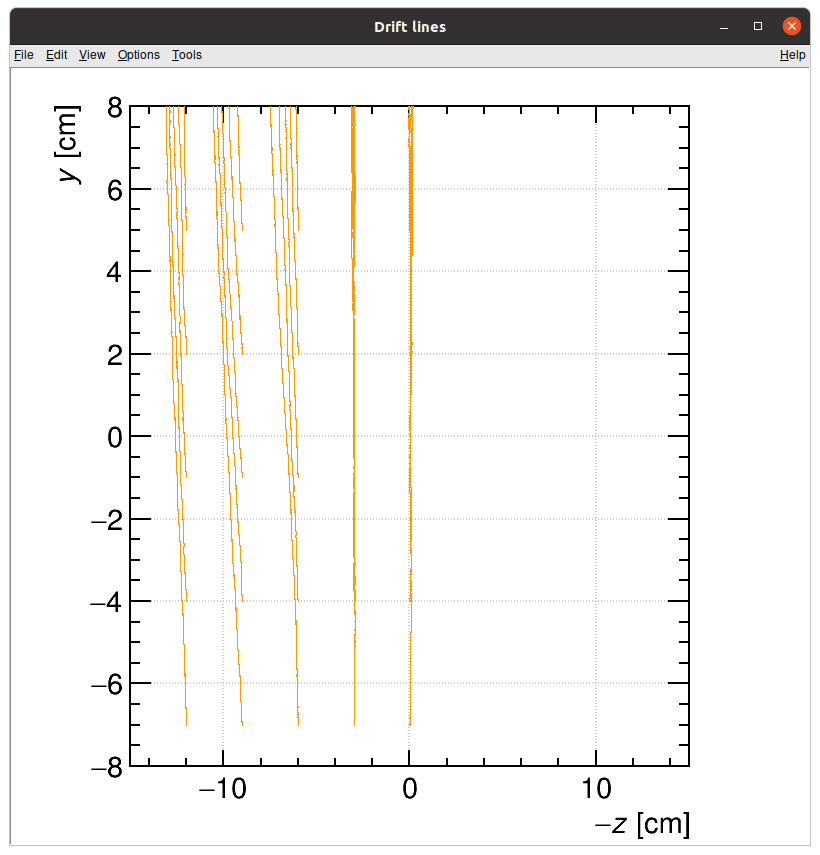
\includegraphics[width=0.5\textwidth]{map_9010_gen.png}
			\caption{Example of map generation. \textcolor{red}{Swap for better image, correct coordinates.}}
			\label{fig:map9010gen}
		\end{figure}
		
		\begin{figure}[H]
			\centering
			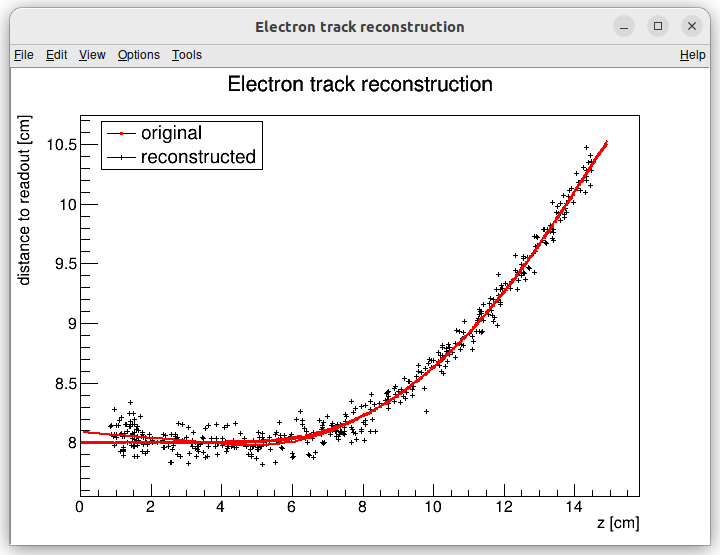
\includegraphics[width=0.5\textwidth]{9010_reco.png}
			\caption{Example reconstruction with the~map. \textcolor{red}{Swap for better image, correct coordinates.}}
			\label{fig:9010reco}
		\end{figure}
		
		\subsection{Gradient Descent Search}
		\label{sec:grad}			
			The~first implemented method of reconstruction uses a~gradient descent search to find an~approximation of the~point in detector space with given mean readout coordinates. Gradient descent is an~iterative minimization algorithm for multivariate functions. Let $R\in\mathcal{R}$ be a~point in the~readout space; we want to find a~point $D = (x,y,z) \in\mathcal{D}$ in the~detector space such that 
				\begin{equation}
					\overbar{\mathcal{M}}(D) = R = (x'_R,y'_R,t_R).
				\end{equation}
			We define a~function~$f_R$ in the~readout space as a~modified distance in this space:
				\begin{equation}
					f_R(x',y',t) = \sqrt{(x'-x'_R)^2+(y'-y'_R)^2+v_d^2(t-t_R)^2},
				\end{equation}
			where $v_d$ is an~approximation of the~drift velocity in the~\ac{TPC}, obtained from the~reconstruction in Section~\ref{sec:trackfirst} (\textcolor{red}{there will be an image with the~linear fit there}). We make the~initial guess (\textcolor{red}{actually in the~original code we just take $z=0$}):
				\begin{equation}
					D_0 = (x'_R,y'_R,v_dt).
				\end{equation}
			Assuming we have the $n$-th estimate $D_n$, we calculate an~approximation of the~$i$-th component of the~gradient of $f_R\circ\overbar{\mathcal{M}}$:
				\begin{equation}
					\nabla(f_R\circ\overbar{\mathcal{M}})^i \approx \frac{f_R(\overbar{\mathcal{M}}(D_n+s\cdot e^i))-f_R(\overbar{\mathcal{M}}(D_n-s\cdot e^i))}{2s},
				\end{equation}
			where $s$ is a~number and $e^i\in\mathcal{D}$ is the~$i$-th coordinate vector. The~number $s$ should be sufficiently small; initially, we set it as a~fraction of the~map's grid spacing $s = \frac{l}{10}$. During the~minimization, we check that $f_R(\overbar{\mathcal{M}}(D_n))<10s$ at all times. \textcolor{red}{When using trilinear interpolation, it would be more efficient to calculate the~gradient explicitly ($\pm$ same result). This could be implemented inside the~\textit{Field} template class.} The~next estimate can be calculated as follows:
				\begin{equation}
					D_{n+1} = D_n - \gamma \nabla(f_R\circ\overbar{\mathcal{M}})(D_n),
				\end{equation}
			where $\gamma\in\mathbb{R}^+$ is the~damping coefficient. It should be set to a~small enough value to ensure convergence, but large enough for sufficient converging speed. The~minimization stops either when the error $f_R(\overbar{\mathcal{M}}(D_n))$ drops below a~specified value or when the~number of iterations exceeds 1000 (in this case, a~message is printed into the~console).
			The parameters of this method could be further optimized (e.g., a~better choice of $\gamma$, \textcolor{red}{gradient computation}); instead, we later decided to use the~interpolation in the~inverse grid described in the~next section.
			
			\textcolor{red}{Measure reconstruction duration and compare it with the~inverse grid interpolation? Also compare the~result? Not sure if this has to be cited.}
		
		\subsection{Interpolation in the~Inverse Grid}
		\label{sec:interpol}
			\textcolor{red}{Interpolating between known points in the~readout space. Gaussian elimination, multivariate polynomial. Benefits compared to the~gradient descent search method (one-time computation for the~whole map is easy to achieve if needed).}
			
			The~currently used reconstruction method is the~interpolation in the~inverse grid. Rather than attempting to invert the~trilinearly interpolated map as in the~previous section, we take advantage of the~fact that the~map $\overbar{\mathcal{M}}$ is one-to-one. Since we have simulated values of this map on a~regular grid in the~detector space $\mathcal{D}$, we also know the~inverse map $\overbar{\mathcal{M}}^{-1}$ on the~irregular inverse grid in the~readout space $\mathcal{R}$. To get an~approximation of the~inverse map in the~entire readout space, we can use interpolation.
			
			Since the~inverse grid is irregular, we cannot use trilinear interpolation. Since the~simulated map is dense enough to give us a~good approximation considering the~size of our pads, we can use a~similar approach (more complicated and computationally heavy alternative would be the~natural neighbor interpolation). As shown in the~equation~\ref{eq:trilinpoly} in Section~\ref{sec:trilin}, trilinear interpolation can be expressed as a~polynomial:
				\begin{equation}
					\widehat{f}(x,y,z) = axyz + bxy + cxz + dyz + ex + fy + gz + h,
				\end{equation}
			where $a,b,c,d,e,f,g,h$ are coefficients determined uniquely by the~values of the~function on the~vertices of the~interpolation cube. We can generalize this for a~function known on an~irregular grid. If we know the~value of a~function in any eight points, we can take a~system of eight linear equations
				\begin{equation}
					\begin{pmatrix}
						x_1 y_1 z_1 & x_1 y_1 & x_1 z_1 & y_1 z_1 & x_1 & y_1 & z_1 & 1\\
						\vdots & \vdots & \vdots & \vdots & \vdots & \vdots & \vdots & \vdots\\
						x_8 y_8 z_8 & x_8 y_8 & x_8 z_8 & y_8 z_8 & x_8 & y_8 & z_8 & 1
					\end{pmatrix}
					\begin{pmatrix}
						a\\
						\vdots\\
						h
					\end{pmatrix}
					=
					\begin{pmatrix}
						f(x_1,y_1,z_1)\\
						\vdots\\
						f(x_8,y_8,z_8)
					\end{pmatrix},
				\end{equation}
			which gives us a~unique solution for the~coefficients for most values of $(x_n, y_n, z_n)$ and $f(x_n,y_n,z_n)$, where $n\in\{1,\ldots,8\}$.
			
			Using this approach introduces a~small problem: finding the~correct pseudocell (i.e., the image of eight vertices forming a~cubic cell in the~regular grid) in the~inverse grid. The~eight irregularly spaced vertices of this pseudocell do not define a~unique solid body, so there is no straightforward way to divide $\mathcal{R}$ into pseudocells using only these vertices.
			
			\textcolor{red}{We are currently ignoring this problem and performing binary search along $x$, $y$, $z$ (in this order). It shouldn't matter too much because the~70/30 map doesn't cause such a big distortion and was even accidentally extrapolated for all $z$ different from the central plane.}
			\textcolor{red}{Interpolation should be generally faster than the~gradient descent since we don't need to iterate. We also don't need to optimize it to improve performance, if it's too slow we can even calculate the~coefficients for the~entire map before reconstruction.}
			
			\begin{figure}[H]
				\centering
				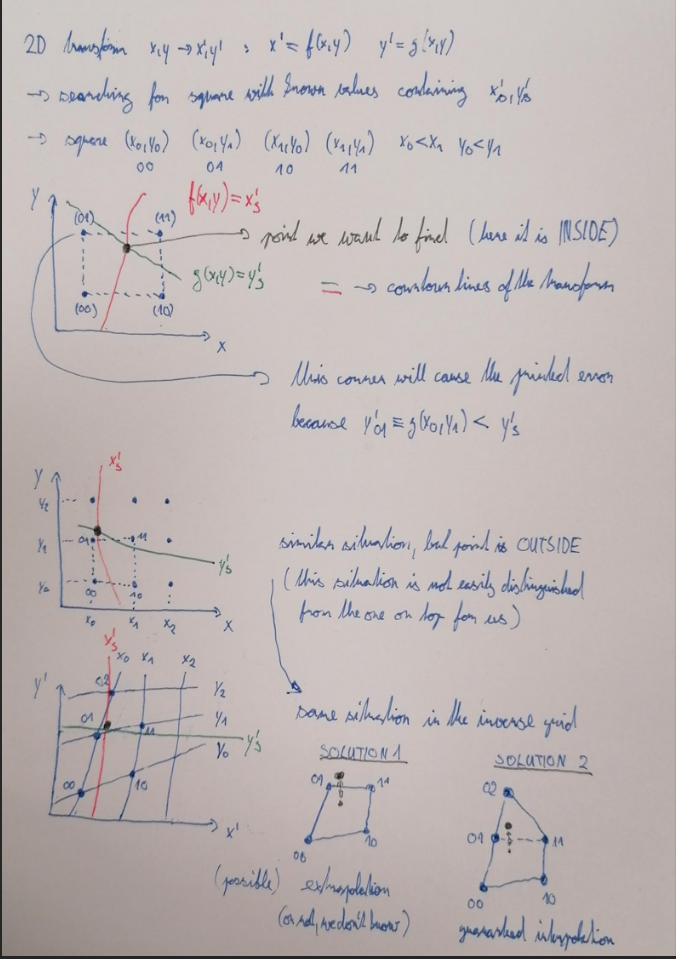
\includegraphics[width=0.8\textwidth]{interpol.png}
				\caption{Selection of the~points for interpolation. \textcolor{red}{Create better images; use the~explanation interpolation vs. extrapolation strange property. Solution~2 probably does not make much sense.}}
				\label{fig:interpol}
			\end{figure}
		
	\section{Discrete Reconstruction}
		\textcolor{red}{Reconstruction with pads and time bins. Maybe testing different pads. Mapping the~center of the pad (along with the~midpoint of the~time bin) isn't necessarily the~best approach since it might not correspond to the~average parameters of an~electron with these readout parameters (insignificant?).}
		
		\textcolor{red}{It is also possible to make this a~subsection of the~map, making the previous subsections parts of a~new subsection 'Map Inversion'.}